
\section{Introduction}
In the lazy/NTK regime, training deep neural networks linearizes and reduces to kernel regression with an (approximately) fixed Gram matrix~\cite{jacot2018neural}. To reduce parameters, one can factorize weights as \(W=LR^\top\) with \(r\ll\min\{n,m\}\); a central question is whether such factorizations preserve favorable optimization and convergence~\cite{zhang2025structuredbalancedmulticomponentmultilayer}. We combine this with the random-feature lazy regime: we freeze the feature (left) directions and train only the readout (right) factors into a bottleneck of dimension \(r\) per layer. That combination defines the RF-LR architecture studied in this paper: RF-LR freezes random feature directions and trains only linear readouts (and biases) into a bottleneck of dimension \(r\ll N\) at each layer. This paper asks: \emph{how do depth \(L\) and bottleneck dimension \(r\) control conditioning-relevant scales for optimization under the NTK perspective?} We adopt the standard NTK setup (ReLU activation, isotropic Gaussian initialization, sequential infinite-width limit) and analyze the induced kernel at initialization.

The architecture stacks high-then-low width layers with a bottleneck \(r\ll n_1\); we train readouts and biases while keeping feature directions frozen. In the kernel regime, the Gram matrix spectrum controls optimization rates~\cite{jacot2018neural,cao2020understandingspectralbiasdeep}. We characterize limiting kernels and spectra under a composition-of-GPs view in the sequential infinite-width limit. Figure~\ref{fig:RF-LR_architecture} illustrates the layout.

\begin{figure}[htbp]
    \centering
    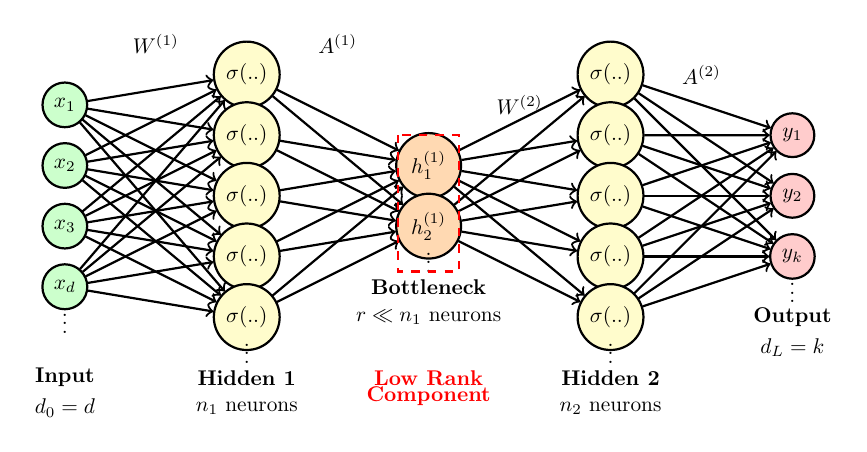
\begin{tikzpicture}[
        scale=0.77, transform shape,
        node distance=2cm and 3cm,
        neuron/.style={circle, draw, fill=blue!20, minimum size=15pt},
        input/.style={circle, draw, fill=green!20, minimum size=15pt},
        output/.style={circle, draw, fill=red!20, minimum size=15pt},
        hidden/.style={circle, draw, fill=yellow!20, minimum size=15pt},
        bottleneck/.style={circle, draw, fill=orange!30, minimum size=15pt},
        thick
    ]
    % Input layer
    \node[input] (x1) at (0,2) {$x_1$};
    \node[input] (x2) at (0,1) {$x_2$};
    \node[input] (x3) at (0,0) {$x_3$};
    \node[input] (xd) at (0,-1) {$x_d$};
    \node at (0,-1.5) {$\vdots$};
    % First hidden layer
    \node[hidden] (h11) at (3,2.5) {$\sigma(..)$};
    \node[hidden] (h12) at (3,1.5) {$\sigma(..)$};
    \node[hidden] (h13) at (3,0.5) {$\sigma(..)$};
    \node[hidden] (h14) at (3,-0.5) {$\sigma(..)$};
    \node[hidden] (h15) at (3,-1.5) {$\sigma(..)$};
    \node at (3,-2) {$\vdots$};
    % Bottleneck layer (low rank)
    \node[bottleneck] (b1) at (6,1) {$h_1^{(1)}$};
    \node[bottleneck] (b2) at (6,0) {$h_2^{(1)}$};
    \node at (6,-0.5) {$\vdots$};
    % Second hidden layer
    \node[hidden] (h21) at (9,2.5) {$\sigma(..)$};
    \node[hidden] (h22) at (9,1.5) {$\sigma(..)$};
    \node[hidden] (h23) at (9,0.5) {$\sigma(..)$};
    \node[hidden] (h24) at (9,-0.5) {$\sigma(..)$};
    \node[hidden] (h25) at (9,-1.5) {$\sigma(..)$};
    \node at (9,-2) {$\vdots$};
    % Output layer
    \node[output] (y1) at (12,1.5) {$y_1$};
    \node[output] (y2) at (12,0.5) {$y_2$};
    \node[output] (yk) at (12,-0.5) {$y_k$};
    \node at (12,-1) {$\vdots$};
    % Connections input to first hidden
    \foreach \i in {1,2,3,d} {
        \foreach \j in {11,12,13,14,15} {
            \draw[->] (x\i) -- (h\j);
        }
    }
    % Connections first hidden to bottleneck
    \foreach \i in {11,12,13,14,15} {
        \foreach \j in {1,2} {
            \draw[->] (h\i) -- (b\j);
        }
    }
    % Connections bottleneck to second hidden
    \foreach \i in {1,2} {
        \foreach \j in {21,22,23,24,25} {
            \draw[->] (b\i) -- (h\j);
        }
    }
    % Connections second hidden to output
    \foreach \i in {21,22,23,24,25} {
        \foreach \j in {1,2,k} {
            \draw[->] (h\i) -- (y\j);
        }
    }
    % Layer labels
    \node at (0,-2.5) {\textbf{Input}};
    \node at (0,-3) {$d_0 = d$};
    \node at (3,-2.5) {\textbf{Hidden 1}};
    \node at (3,-3) {$n_1$ neurons};
    \node at (6,-1) {\textbf{Bottleneck}};
    \node at (6,-1.5) {$r \ll n_1$ neurons};
    \node at (9,-2.5) {\textbf{Hidden 2}};
    \node at (9,-3) {$n_2$ neurons};
    \node at (12,-1.5) {\textbf{Output}};
    \node at (12,-2) {$d_L = k$};
    % Mathematical notation
    \node at (1.5,3) {$\bm{W}^{(1)}$};
    \node[yshift=2cm] at (4.5,1) {$\bm{A}^{(1)}$};
    \node at (7.5,2) {$\bm{W}^{(2)}$};
    \node[yshift=2cm] at (10.5,0.5) {$\bm{A}^{(2)}$};
    % Highlight low rank structure
    \draw[red, thick, dashed] (5.5,1.5) rectangle (6.5,-0.75);
    \node[red] at (6,-2.5) {\textbf{Low Rank}};
    \node[red] at (6,-2.8) {\textbf{Component}};
    \end{tikzpicture}
    \caption{RF-LR: low-rank bottleneck (red dashed) reduces width from \(n_1\) to \(r\); readouts trained, feature directions frozen.}
    \label{fig:RF-LR_architecture}
\end{figure}

The NTK framework~\cite{jacot2018neural} characterises infinitely wide networks as kernel methods. Extensions include finite-width corrections~\cite{arora2019exact,dyer2019asymptoticswidenetworksfeynman}, depth scaling~\cite{yang2019scaling,terjek2022depth}, and, in the extensive-width regime \(n\sim N^2\) with layers in the RMT limit, limits for Gram spectra~\cite{benigni2025eigenvaluedistributionneuraltangent}. Low-rank architectures cut parameters and change optimisation dynamics~\cite{sainath2013low,novikov2015tensorizing,arora2018optimization}. Freezing feature directions isolates the bottleneck dimension \(r\) as the main control parameter. LoRA-style theory places low-rank fine-tuning between kernel and feature-learning regimes~\cite{dayi2024gradientdynamicslowrankfinetuning,jang2024loratrainingntkregime}. For ReLU kernels, Bietti and Bach~\cite{bietti2021deepequalsshallowrelu} showed that deep and shallow networks can induce the same RKHS via endpoint expansions. We combine Fisher--Kibble decoupling~\cite{fisher1915probable,hotelling1953new} with Puiseux analysis near \(\rho=1\) to get the same for the three-layer RF-LR mean kernel.

For MLPs at the edge of chaos, depth drives correlations toward \(1\); layerwise kernels become nearly constant and the deep mean kernel tends to rank-one~\cite{terjek2025mlpsateoc,pmlr-v163-hayou22a}. The NTK Gram matrix's maximum eigenvalue scales linearly with depth, which can make training unstable. The same correlation alignment holds in RF-LR, but our proxy kernel has bounded \(\lambda_{\max}\), so a fixed learning rate stays valid. The mean kernel's infinite-depth limit still collapses after centering unless time or learning rate is rescaled (Appendix~\ref{appendix:infinite-depth-limit}). Freezing random features removes cross-layer dependencies present in fully trained nets; with Fisher--Kibble decoupling this yields explicit formulas and a path to joint large-\(n\) regimes in the RMT framework~\cite{benigni2025eigenvaluedistributionneuraltangent}. Theorem~\ref{thm:ntk_recursion} suggests organising finite-width corrections as an expansion in \(r\). Future work may address tensor programs~\cite{yang2020tensorprogramsiineural} and depth-dependent NTK spectra for MLPs at EOC~\cite{terjek2025mlpsateoc}, with explicit bottleneck scaling.

In the lazy/NTK regime, gradient flow reduces to kernel regression with an (approximately) fixed kernel~\cite{jacot2018neural}, and the spectrum of that kernel governs convergence and stability; we characterise the RF-LR NTK in the sequential infinite-width limit and establish the following contributions.
\begin{itemize}
    \item \textbf{Explicit NTK recursion and closed form.} We derive the infinite-width NTK recursion for RF-LR with an explicit \(1/r\) factor at each bottleneck layer and a closed-form \(L\)-layer expansion (Theorem~\ref{thm:ntk_recursion}, Corollary~\ref{cor:general_L_layer_ntk}).
    \item \textbf{Depth scaling and condition number.} For the deterministic proxy kernel we prove sharp depth scaling: correlation alignment \(1-\rho_k=\Theta(k^{-2})\) (the same as for full-width MLPs at the edge of chaos~\cite{terjek2025mlpsateoc,pmlr-v163-hayou22a}), kernel saturation to a fixed point, and diagonal--off-diagonal gap \(\asymp 1/(rk)\) (Theorem~\ref{thm:rflr-depth-scaling-mean}). We prove a condition-number \emph{lower bound} \(\kappa\ge\Omega(r\cdot L)\) for the proxy Gram in general (Proposition~\ref{prop:condition-number-depth}), and \emph{exact} conditioning \(\kappa_\perp=1\) or \(\kappa_\perp=1+o(1)\) for equicorrelated or high-dimensional spherical data (Corollary~\ref{cor:conditioning-equicorrelated-highdim}). Under a fixed parameter budget \(O(NLr)\), depth and rank thus trade off from a conditioning perspective.
    \item \textbf{RKHS equivalence (three layers).} We show that the mean three-layer RF-LR kernel induces the same RKHS as the shallow ReLU kernel (Corollary~\ref{thm:no_rkhs_advantage}): the bottleneck does not shrink the kernel-regime function class, while reducing trainable parameters from \(O(LN^2)\) to \(O(LrN)\) per layer. The proof uses Fisher--Kibble decoupling and a Puiseux expansion at the endpoint; extension to \(L\ge 4\) remains open.
    \item \textbf{Numerical experiments.} Appendix~\ref{sec:experiments} presents deterministic and finite-width experiments that confirm the depth scaling (Theorem~\ref{thm:rflr-depth-scaling-mean}), equicorrelated and high-dimensional conditioning (Corollary~\ref{cor:conditioning-equicorrelated-highdim}), and proxy--empirical concentration (Theorem~\ref{thm:equicorrelated-op-bound}); non-equicorrelated data illustrate the \(\kappa\ge\Omega(r\cdot L)\) lower bound (Proposition~\ref{prop:condition-number-depth}).
\end{itemize}
All condition-number bounds refer to the proxy Gram matrix; we give a rigorous proxy--empirical bound on \(\mathbf{1}^\perp\) for equicorrelated data (Theorem~\ref{thm:equicorrelated-op-bound}). Proof sketch: Appendix~\ref{appendix:techniques-proof-sketch}.

\paragraph{Paper organization.}
Section~\ref{sec:network-definition} defines the RF-LR architecture, training policy, EOC parameterization, and the base and derivative kernels. Section~\ref{sec:recursion} states the infinite-width NTK recursion and its closed-form \(L\)-layer expansion. Section~\ref{sec:depth-scaling} gives depth scaling for the deterministic proxy kernel and condition-number bounds (proxy and, for equicorrelated data, empirical). Section~\ref{sec:no-rkhs-advantage} proves that the three-layer mean RF-LR kernel induces the same RKHS as the shallow ReLU kernel via Fisher--Kibble decoupling and Puiseux analysis. 
